% Options for packages loaded elsewhere
\PassOptionsToPackage{unicode}{hyperref}
\PassOptionsToPackage{hyphens}{url}
%
\documentclass[
  11pt,
]{article}
\usepackage{amsmath,amssymb}
\usepackage{iftex}
\ifPDFTeX
  \usepackage[T1]{fontenc}
  \usepackage[utf8]{inputenc}
  \usepackage{textcomp} % provide euro and other symbols
\else % if luatex or xetex
  \usepackage{unicode-math} % this also loads fontspec
  \defaultfontfeatures{Scale=MatchLowercase}
  \defaultfontfeatures[\rmfamily]{Ligatures=TeX,Scale=1}
\fi
\usepackage{lmodern}
\ifPDFTeX\else
  % xetex/luatex font selection
\fi
% Use upquote if available, for straight quotes in verbatim environments
\IfFileExists{upquote.sty}{\usepackage{upquote}}{}
\IfFileExists{microtype.sty}{% use microtype if available
  \usepackage[]{microtype}
  \UseMicrotypeSet[protrusion]{basicmath} % disable protrusion for tt fonts
}{}
\makeatletter
\@ifundefined{KOMAClassName}{% if non-KOMA class
  \IfFileExists{parskip.sty}{%
    \usepackage{parskip}
  }{% else
    \setlength{\parindent}{0pt}
    \setlength{\parskip}{6pt plus 2pt minus 1pt}}
}{% if KOMA class
  \KOMAoptions{parskip=half}}
\makeatother
\usepackage{xcolor}
\usepackage[margin=1in]{geometry}
\usepackage{color}
\usepackage{fancyvrb}
\newcommand{\VerbBar}{|}
\newcommand{\VERB}{\Verb[commandchars=\\\{\}]}
\DefineVerbatimEnvironment{Highlighting}{Verbatim}{commandchars=\\\{\}}
% Add ',fontsize=\small' for more characters per line
\usepackage{framed}
\definecolor{shadecolor}{RGB}{248,248,248}
\newenvironment{Shaded}{\begin{snugshade}}{\end{snugshade}}
\newcommand{\AlertTok}[1]{\textcolor[rgb]{0.94,0.16,0.16}{#1}}
\newcommand{\AnnotationTok}[1]{\textcolor[rgb]{0.56,0.35,0.01}{\textbf{\textit{#1}}}}
\newcommand{\AttributeTok}[1]{\textcolor[rgb]{0.13,0.29,0.53}{#1}}
\newcommand{\BaseNTok}[1]{\textcolor[rgb]{0.00,0.00,0.81}{#1}}
\newcommand{\BuiltInTok}[1]{#1}
\newcommand{\CharTok}[1]{\textcolor[rgb]{0.31,0.60,0.02}{#1}}
\newcommand{\CommentTok}[1]{\textcolor[rgb]{0.56,0.35,0.01}{\textit{#1}}}
\newcommand{\CommentVarTok}[1]{\textcolor[rgb]{0.56,0.35,0.01}{\textbf{\textit{#1}}}}
\newcommand{\ConstantTok}[1]{\textcolor[rgb]{0.56,0.35,0.01}{#1}}
\newcommand{\ControlFlowTok}[1]{\textcolor[rgb]{0.13,0.29,0.53}{\textbf{#1}}}
\newcommand{\DataTypeTok}[1]{\textcolor[rgb]{0.13,0.29,0.53}{#1}}
\newcommand{\DecValTok}[1]{\textcolor[rgb]{0.00,0.00,0.81}{#1}}
\newcommand{\DocumentationTok}[1]{\textcolor[rgb]{0.56,0.35,0.01}{\textbf{\textit{#1}}}}
\newcommand{\ErrorTok}[1]{\textcolor[rgb]{0.64,0.00,0.00}{\textbf{#1}}}
\newcommand{\ExtensionTok}[1]{#1}
\newcommand{\FloatTok}[1]{\textcolor[rgb]{0.00,0.00,0.81}{#1}}
\newcommand{\FunctionTok}[1]{\textcolor[rgb]{0.13,0.29,0.53}{\textbf{#1}}}
\newcommand{\ImportTok}[1]{#1}
\newcommand{\InformationTok}[1]{\textcolor[rgb]{0.56,0.35,0.01}{\textbf{\textit{#1}}}}
\newcommand{\KeywordTok}[1]{\textcolor[rgb]{0.13,0.29,0.53}{\textbf{#1}}}
\newcommand{\NormalTok}[1]{#1}
\newcommand{\OperatorTok}[1]{\textcolor[rgb]{0.81,0.36,0.00}{\textbf{#1}}}
\newcommand{\OtherTok}[1]{\textcolor[rgb]{0.56,0.35,0.01}{#1}}
\newcommand{\PreprocessorTok}[1]{\textcolor[rgb]{0.56,0.35,0.01}{\textit{#1}}}
\newcommand{\RegionMarkerTok}[1]{#1}
\newcommand{\SpecialCharTok}[1]{\textcolor[rgb]{0.81,0.36,0.00}{\textbf{#1}}}
\newcommand{\SpecialStringTok}[1]{\textcolor[rgb]{0.31,0.60,0.02}{#1}}
\newcommand{\StringTok}[1]{\textcolor[rgb]{0.31,0.60,0.02}{#1}}
\newcommand{\VariableTok}[1]{\textcolor[rgb]{0.00,0.00,0.00}{#1}}
\newcommand{\VerbatimStringTok}[1]{\textcolor[rgb]{0.31,0.60,0.02}{#1}}
\newcommand{\WarningTok}[1]{\textcolor[rgb]{0.56,0.35,0.01}{\textbf{\textit{#1}}}}
\usepackage{longtable,booktabs,array}
\usepackage{calc} % for calculating minipage widths
% Correct order of tables after \paragraph or \subparagraph
\usepackage{etoolbox}
\makeatletter
\patchcmd\longtable{\par}{\if@noskipsec\mbox{}\fi\par}{}{}
\makeatother
% Allow footnotes in longtable head/foot
\IfFileExists{footnotehyper.sty}{\usepackage{footnotehyper}}{\usepackage{footnote}}
\makesavenoteenv{longtable}
\usepackage{graphicx}
\makeatletter
\def\maxwidth{\ifdim\Gin@nat@width>\linewidth\linewidth\else\Gin@nat@width\fi}
\def\maxheight{\ifdim\Gin@nat@height>\textheight\textheight\else\Gin@nat@height\fi}
\makeatother
% Scale images if necessary, so that they will not overflow the page
% margins by default, and it is still possible to overwrite the defaults
% using explicit options in \includegraphics[width, height, ...]{}
\setkeys{Gin}{width=\maxwidth,height=\maxheight,keepaspectratio}
% Set default figure placement to htbp
\makeatletter
\def\fps@figure{htbp}
\makeatother
\setlength{\emergencystretch}{3em} % prevent overfull lines
\providecommand{\tightlist}{%
  \setlength{\itemsep}{0pt}\setlength{\parskip}{0pt}}
\setcounter{secnumdepth}{5}
\usepackage{setspace}
\doublespacing
\usepackage{setspace}
\ifLuaTeX
  \usepackage{selnolig}  % disable illegal ligatures
\fi
\usepackage{bookmark}
\IfFileExists{xurl.sty}{\usepackage{xurl}}{} % add URL line breaks if available
\urlstyle{same}
\hypersetup{
  pdftitle={Final Project},
  pdfauthor={Hwanho Kim},
  hidelinks,
  pdfcreator={LaTeX via pandoc}}

\title{Final Project}
\author{Hwanho Kim}
\date{2025-04-26}

\begin{document}
\maketitle

\section{Abstract}\label{abstract}

This project predicts the probability that each stock will have a
positive return in the future by using the hierarchical Bayesian model.
In the data, each stock will have 1 if that stock had a positive return
in that period, 0 otherwise. I treat the outcome of the observed stocks
as Bernoulli outcomes, and the probability of the stock is affected by
the industry to which the stock belongs. Each stock's probability of a
positive return is assumed to arise from a sector-level Beta
distribution with the parameters reflecting market uncertainty. The
Exploratory Data Analysis process will show the differences not only
among stocks but also among sectors, and we can summarize our data
numerically and graphically. I fit the model using Markov Chain Monte
Carlo (MCMC) methods with JAGS and diagnose convergence. Posterior
analysis allows us to estimate the probability that each sector offers
the best investment opportunities, and to distinguish the most promising
stock within each sector.

\section{Data}\label{data}

\subsection{Input Data Description}\label{input-data-description}

The dataset shows us the return record of 50 stocks in different
periods, and each stock belongs to one of 5 sectors. Individual stocks
are observed over 30 periods, and they have 1 if that stock in a
specific sector had a positive return, 0 otherwise. The dataset has 3
columns: sectors, stock, and flip, and each row represents whether a
stock within a specific sector had a positive return in that period or
not. The dataset has 5 sectors, and each sector contains 10 stocks.
Thus, there are 1,5000 observations total in the dataset (50 stocks x 30
periods each).

We have only 30 periods for each stock, which is a relatively small
number of stocks to clarify the uncertainty in parameter estimates.
Also, we assume that returns within each stock are independently and
identically distributed. These limitations of the dataset enable our
model to process easily and plausibly.

\subsection{Explanatory Data Analysis}\label{explanatory-data-analysis}

In this project, the goal of EDA was to summarize the dataset in terms
of market, sector (industry), and stock. Overall, the dataset consists
of 1,500 observations, each binary outcome representing whether or not a
specific stock in a certain sector had a positive return during the
given period.

\begin{longtable}[]{@{}rrr@{}}
\caption{Table 1: Summary of Flip Outcomes}\tabularnewline
\toprule\noalign{}
Flip & Count & Proportion \\
\midrule\noalign{}
\endfirsthead
\toprule\noalign{}
Flip & Count & Proportion \\
\midrule\noalign{}
\endhead
\bottomrule\noalign{}
\endlastfoot
0 & 721 & 0.4807 \\
1 & 779 & 0.5193 \\
\end{longtable}

In a market aspect, I count the number of 0 and 1, and compare them on a
proportion scale. In this market, 721 stocks had negative returns, and
779 stocks had positive returns. In other words, 48.067 percent of
stocks had negative returns, and 51.933 percent of stocks had positive
returns.

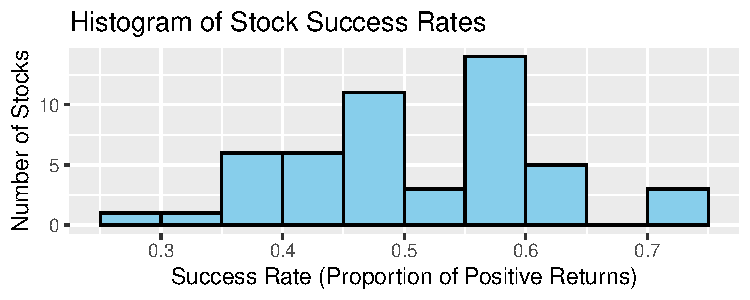
\includegraphics{Final-Project_files/figure-latex/unnamed-chunk-2-1.pdf}

In the stock aspect, individual stocks show various success rates,
ranging approximately from 0.33 to 0.73. The wide probability range
demonstrates that each stock have a different success rate, and the
probability of a positive return for each stock is affected by other
factors. In the histogram, the success rate is more focused on the
interval {[}0.4, 0.5{]} and {[}0.5, 0.6{]}. We can conclude that each
stock has a different probability of positive return, and the
distribution is focused on a near 0.5 success rate interval.

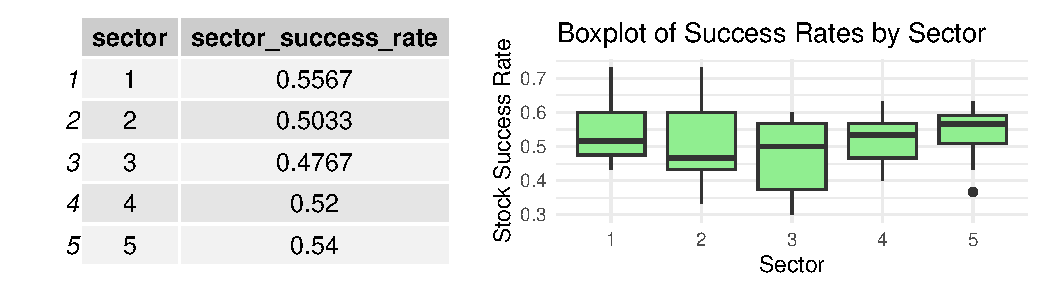
\includegraphics{Final-Project_files/figure-latex/unnamed-chunk-3-1.pdf}
In the sector aspect, they have quite different rates of success, even
thoughthe rates are close with 0.5. The table and box plot have
different means because I try to group the data by sector, and calculate
the mean for the table while I use summary of data which is grouped by
sector and plotted as box plot. However, these two clearly show that
different industry affect to the probability of stocks within that.

\section{Model}\label{model}

\subsection{Model Selection}\label{model-selection}

I use a hierarchical Bayesian model to predict the probability that a
stock produces a positive return. The model has three levels: individual
observations, sectors, and the overall market.

\subsubsection{Observation Level}\label{observation-level}

\(y_{ijt} \sim Bernouli(\theta_{ij})\) where \(i = {1, 2, 3, .... 10}\),
\(j = {1, 2, 3, 4, 5}\), \(t = {1, 2, 3, ... 30}\)

For each stock i in sector j in period t, \(y_{ijt}\) will have 1 if it
has a positive return.

\(y_{ijt}\) model each flip given the stock's positive return
probability.

\subsubsection{Stock Level}\label{stock-level}

\(\theta_{ij} \sim Beta(\alpha_j, \beta_j)\)

This variable models each stock's success probability inside each
sector.

\(\theta_{ij}\) is the probability of positive return of stock i in
sector j.

\(\alpha_j\) and \(\beta_j\) are parameters controlling the mean and
variance of success rates within sector j.

\subsubsection{Sector Level}\label{sector-level}

\(\alpha_j \sim Gamma(2, 0.1)\), \(\beta_j \sim Gamma(2, 0.1)\)

The parameters \(\alpha_j\) and \(\beta_j\) have weakly informative
priors.

This model uncertainty across sectors.

\subsection{Justification}\label{justification}

This hierarchical structure considers not only the variability of stocks
within the sector but also the variability between sectors, and
parameters are affected by the previous level's parameters. Therefore, a
hierarchical Bayesian model is appropriate for modeling the flip.

\subsection{Model Building}\label{model-building}

I implement the hierarchical Bayesian model using the rjags package in R
to perform Markov Chain Monte Carlo (MCMC) sampling. For the algorithm
setting, I use 3 chains, and 10,000 iterations occur per chain, total of
30,000 iterations. The model will use the first 5,000 iterations as a
Burn-in period. The model will use random starting values for the
parameters. For example, \(\theta_{i,j}\) will be initialized by a
random value from a \(Beta(1, 1)\) distribution.

\subsection{Convergence Diagnostics}\label{convergence-diagnostics}

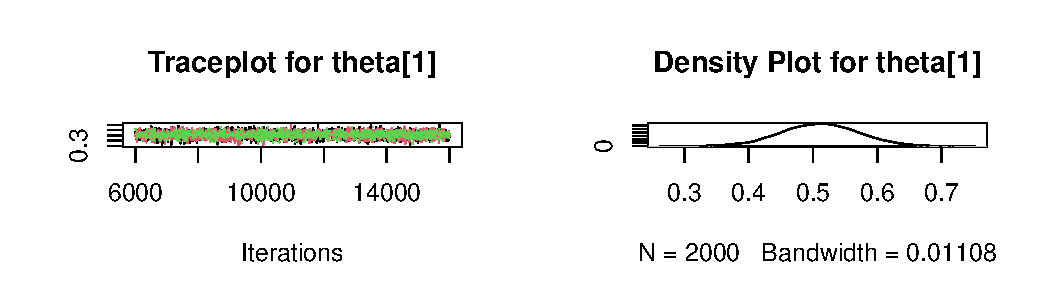
\includegraphics{Final-Project_files/figure-latex/unnamed-chunk-5-1.pdf}
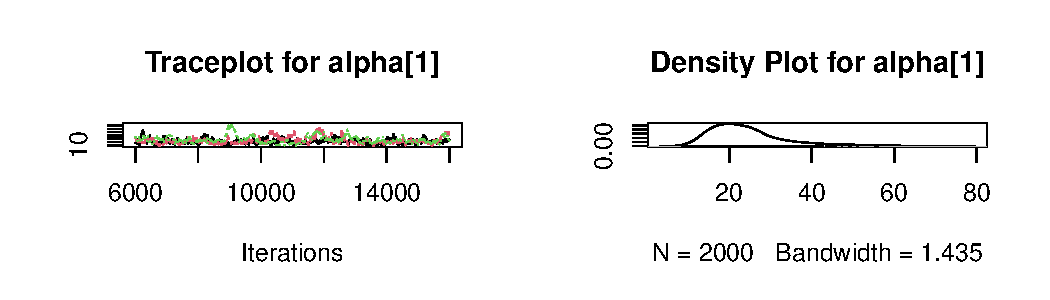
\includegraphics{Final-Project_files/figure-latex/unnamed-chunk-5-2.pdf}
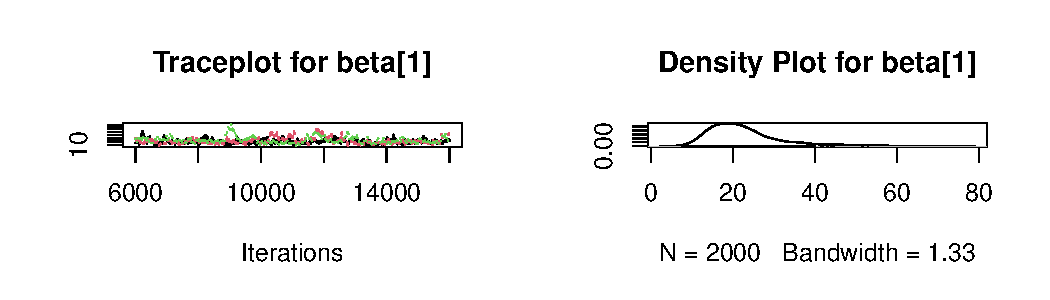
\includegraphics{Final-Project_files/figure-latex/unnamed-chunk-5-3.pdf}
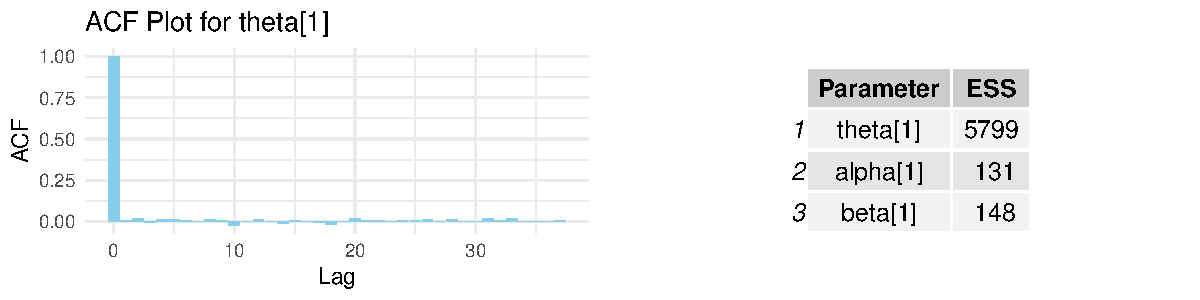
\includegraphics{Final-Project_files/figure-latex/unnamed-chunk-6-1.pdf}

To assess convergence of the MCMC algorithm, we can use the traceplots
and effective sample sizes for all monitored parameters. Originally,
there should be 5 alpha and beta results, and 50 theta results, but I
extracted one example for each parameter now. Three traceplots for
parameters shows the stable and well-mixed behavior across chains
without visible trends, indicating good mixing. ESS (Effective Sample
Sizes) for all parameters were substantially large, ensuring reliable
posterior estimation with minimal autocorrelation, and ACF plot also
prove that this model is effective and converges.

\subsection{Result}\label{result}

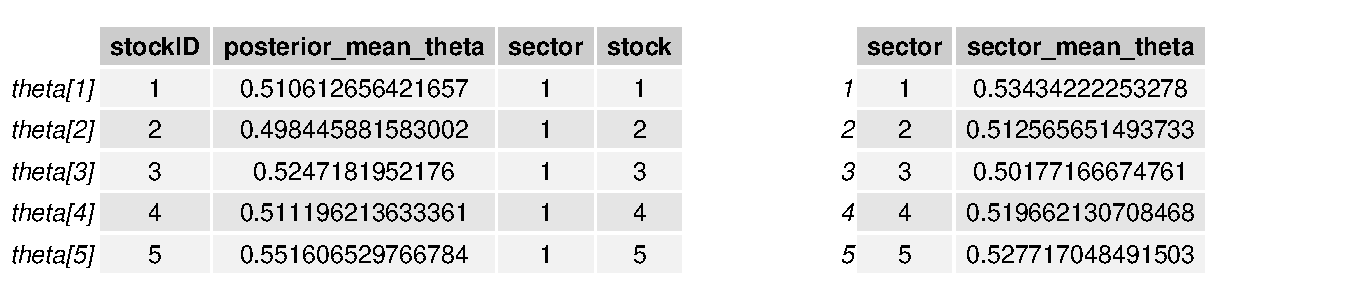
\includegraphics{Final-Project_files/figure-latex/unnamed-chunk-7-1.pdf}
Posterior mean estimates of each stock's probability of a positive
return were calculated based on the MCMC draws. The posterior means
across stocks varied, with most success probabilities ranging from
approximately 0.50 to 0.60. We also can see that average success
probabilities by sectors are almost similar each other in the table
which are near 50 percent. However, sector 1 is the most likely to have
positive return than others.

\begin{longtable}[]{@{}rrrr@{}}
\caption{Table: Best Stock Within Each Sector Based on Posterior Mean
Success Rate}\tabularnewline
\toprule\noalign{}
stockID & posterior\_mean\_theta & sector & stock \\
\midrule\noalign{}
\endfirsthead
\toprule\noalign{}
stockID & posterior\_mean\_theta & sector & stock \\
\midrule\noalign{}
\endhead
\bottomrule\noalign{}
\endlastfoot
8 & 0.6075014 & 1 & 8 \\
15 & 0.6073803 & 2 & 5 \\
26 & 0.5529039 & 3 & 6 \\
31 & 0.5662480 & 4 & 1 \\
41 & 0.5668229 & 5 & 1 \\
\end{longtable}

I extract the stock that has the highest average probability of positive
return for each sector. In sector 1, stock 10 has the highest average
probability and so on.

\section{Conclusion}\label{conclusion}

In this project, we modeled stock returns using a hierarchical Bayesian
framework, treating individual stock returns as Bernoulli trials with
sector-level Beta priors. Exploratory data analysis revealed meaningful
differences across sectors and stocks. Our Bayesian model was fit using
MCMC sampling, and convergence diagnostics confirmed successful
convergence. Posterior analysis identified the sector with the highest
average success probability and the most promising stock within each
sector, providing insights into future investment opportunities.

\section{Appendix}\label{appendix}

\subsection{EDA}\label{eda}

\begin{Shaded}
\begin{Highlighting}[]
\CommentTok{\# 1. Basic table: number of 0s and 1s}
\CommentTok{\# Make the basic table}
\NormalTok{flip\_table }\OtherTok{\textless{}{-}} \FunctionTok{table}\NormalTok{(stock}\SpecialCharTok{$}\NormalTok{flip)}

\CommentTok{\# Convert it into a tidy data frame}
\NormalTok{flip\_summary }\OtherTok{\textless{}{-}} \FunctionTok{data.frame}\NormalTok{(}
  \AttributeTok{flip =} \FunctionTok{as.numeric}\NormalTok{(}\FunctionTok{names}\NormalTok{(flip\_table)),}
  \AttributeTok{count =} \FunctionTok{as.numeric}\NormalTok{(flip\_table),}
  \AttributeTok{proportion =} \FunctionTok{as.numeric}\NormalTok{(flip\_table) }\SpecialCharTok{/} \FunctionTok{sum}\NormalTok{(flip\_table)}
\NormalTok{)}

\CommentTok{\# View the summary table}
\FunctionTok{print}\NormalTok{(flip\_summary)}
\end{Highlighting}
\end{Shaded}

\begin{verbatim}
##   flip count proportion
## 1    0   721  0.4806667
## 2    1   779  0.5193333
\end{verbatim}

\begin{Shaded}
\begin{Highlighting}[]
\CommentTok{\# 2. Mean flip (success rate) per stock}
\NormalTok{stock\_summary }\OtherTok{\textless{}{-}}\NormalTok{ stock }\SpecialCharTok{\%\textgreater{}\%}
  \FunctionTok{group\_by}\NormalTok{(sector, stock) }\SpecialCharTok{\%\textgreater{}\%}
  \FunctionTok{summarize}\NormalTok{(}\AttributeTok{success\_rate =} \FunctionTok{mean}\NormalTok{(flip),}
            \AttributeTok{num\_obs =} \FunctionTok{n}\NormalTok{(),}
            \AttributeTok{.groups =} \StringTok{"drop"}\NormalTok{)}

\CommentTok{\# View the stock summary}
\FunctionTok{print}\NormalTok{(stock\_summary)}
\end{Highlighting}
\end{Shaded}

\begin{verbatim}
## # A tibble: 50 x 4
##    sector stock success_rate num_obs
##     <dbl> <dbl>        <dbl>   <int>
##  1      1     1        0.5        30
##  2      1     2        0.467      30
##  3      1     3        0.533      30
##  4      1     4        0.5        30
##  5      1     5        0.6        30
##  6      1     6        0.467      30
##  7      1     7        0.6        30
##  8      1     8        0.733      30
##  9      1     9        0.433      30
## 10      1    10        0.733      30
## # i 40 more rows
\end{verbatim}

\begin{Shaded}
\begin{Highlighting}[]
\CommentTok{\# 3. Mean flip (success rate) per sector}
\NormalTok{sector\_summary }\OtherTok{\textless{}{-}}\NormalTok{ stock }\SpecialCharTok{\%\textgreater{}\%}
  \FunctionTok{group\_by}\NormalTok{(sector) }\SpecialCharTok{\%\textgreater{}\%}
  \FunctionTok{summarize}\NormalTok{(}\AttributeTok{sector\_success\_rate =} \FunctionTok{mean}\NormalTok{(flip))}

\CommentTok{\# View the sector summary}
\FunctionTok{print}\NormalTok{(sector\_summary)}
\end{Highlighting}
\end{Shaded}

\begin{verbatim}
## # A tibble: 5 x 2
##   sector sector_success_rate
##    <dbl>               <dbl>
## 1      1               0.557
## 2      2               0.503
## 3      3               0.477
## 4      4               0.52 
## 5      5               0.54
\end{verbatim}

\begin{Shaded}
\begin{Highlighting}[]
\CommentTok{\# 4. Plot: Histogram of stock success rates}
\FunctionTok{ggplot}\NormalTok{(stock\_summary, }\FunctionTok{aes}\NormalTok{(}\AttributeTok{x =}\NormalTok{ success\_rate)) }\SpecialCharTok{+}
  \FunctionTok{geom\_histogram}\NormalTok{(}\AttributeTok{binwidth =} \FloatTok{0.05}\NormalTok{, }\AttributeTok{boundary =} \DecValTok{0}\NormalTok{, }\AttributeTok{color =} \StringTok{"black"}\NormalTok{, }\AttributeTok{fill =} \StringTok{"skyblue"}\NormalTok{) }\SpecialCharTok{+}
  \FunctionTok{labs}\NormalTok{(}\AttributeTok{title =} \StringTok{"Histogram of Stock Success Rates"}\NormalTok{,}
       \AttributeTok{x =} \StringTok{"Success Rate (Proportion of Positive Returns)"}\NormalTok{,}
       \AttributeTok{y =} \StringTok{"Number of Stocks"}\NormalTok{)}
\end{Highlighting}
\end{Shaded}

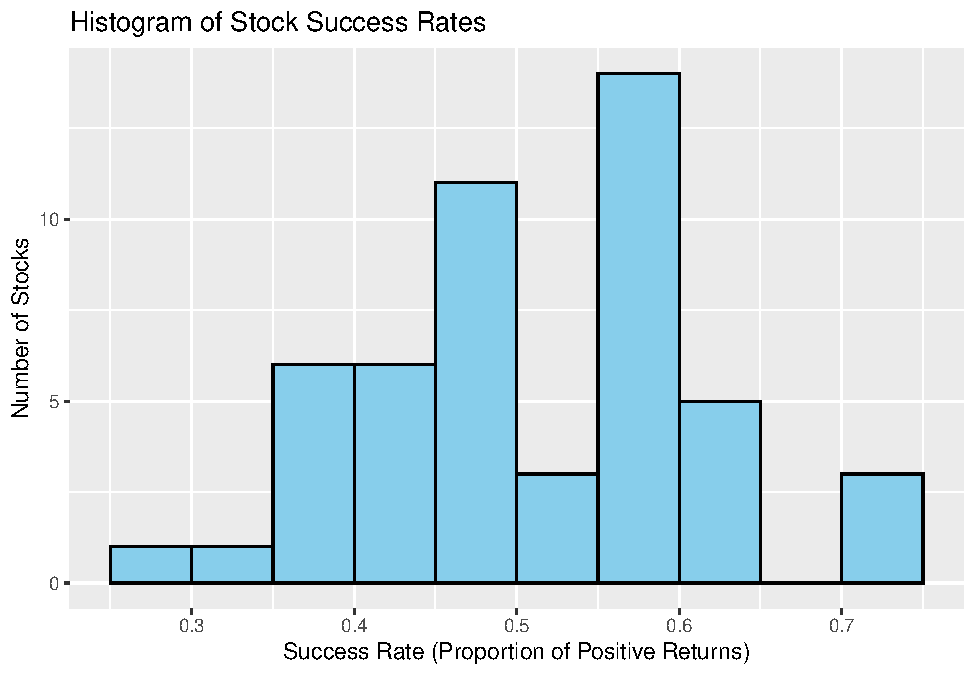
\includegraphics{Final-Project_files/figure-latex/appendix-code-1-1.pdf}

\begin{Shaded}
\begin{Highlighting}[]
\CommentTok{\# 5. Plot: Boxplot of success rates across sectors}
\FunctionTok{ggplot}\NormalTok{(stock\_summary, }\FunctionTok{aes}\NormalTok{(}\AttributeTok{x =} \FunctionTok{factor}\NormalTok{(sector), }\AttributeTok{y =}\NormalTok{ success\_rate)) }\SpecialCharTok{+}
  \FunctionTok{geom\_boxplot}\NormalTok{(}\AttributeTok{fill =} \StringTok{"lightgreen"}\NormalTok{) }\SpecialCharTok{+}
  \FunctionTok{labs}\NormalTok{(}\AttributeTok{title =} \StringTok{"Boxplot of Stock Success Rates by Sector"}\NormalTok{,}
       \AttributeTok{x =} \StringTok{"Sector"}\NormalTok{,}
       \AttributeTok{y =} \StringTok{"Stock Success Rate"}\NormalTok{) }\SpecialCharTok{+}
  \FunctionTok{theme\_minimal}\NormalTok{()}
\end{Highlighting}
\end{Shaded}

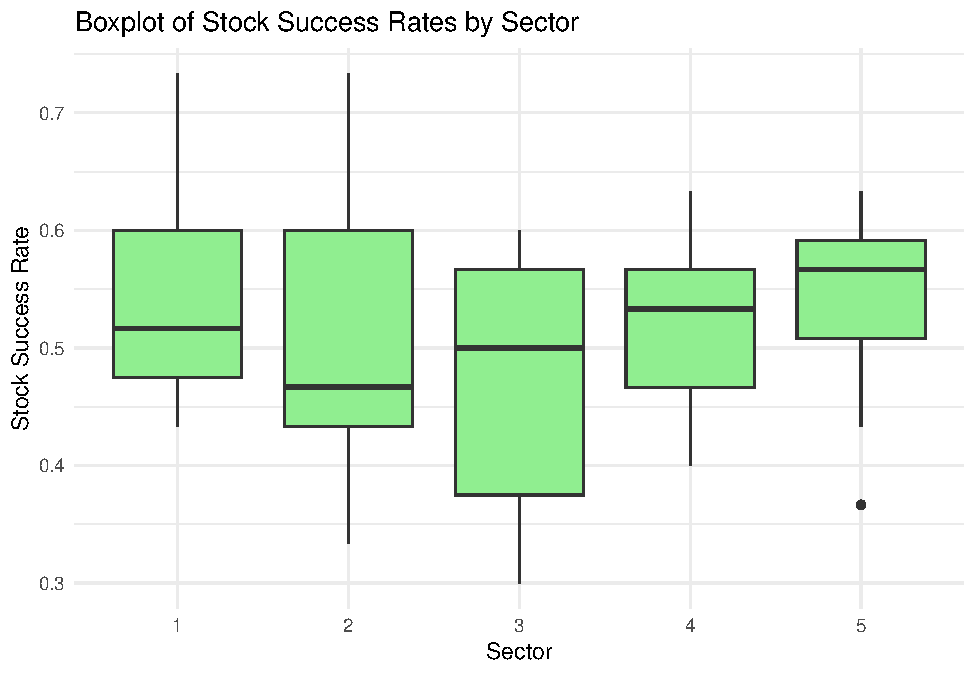
\includegraphics{Final-Project_files/figure-latex/appendix-code-1-2.pdf}

\subsection{Model Building}\label{model-building-1}

\begin{Shaded}
\begin{Highlighting}[]
\CommentTok{\# Set random seed for reproducibility}
\FunctionTok{set.seed}\NormalTok{(}\DecValTok{3303}\NormalTok{)}

\CommentTok{\# Prepare data for JAGS}
\CommentTok{\# Reindex stocks uniquely (sector 1{-}5 and stock 1{-}10 inside)}
\NormalTok{stock}\SpecialCharTok{$}\NormalTok{stockID }\OtherTok{\textless{}{-}}\NormalTok{ (stock}\SpecialCharTok{$}\NormalTok{sector }\SpecialCharTok{{-}} \DecValTok{1}\NormalTok{) }\SpecialCharTok{*} \DecValTok{10} \SpecialCharTok{+}\NormalTok{ stock}\SpecialCharTok{$}\NormalTok{stock}

\CommentTok{\# Number of sectors and stocks}
\NormalTok{n\_sectors }\OtherTok{\textless{}{-}} \FunctionTok{length}\NormalTok{(}\FunctionTok{unique}\NormalTok{(stock}\SpecialCharTok{$}\NormalTok{sector))}
\NormalTok{n\_stocks }\OtherTok{\textless{}{-}} \FunctionTok{length}\NormalTok{(}\FunctionTok{unique}\NormalTok{(stock}\SpecialCharTok{$}\NormalTok{stockID))}

\CommentTok{\# Bundle data for JAGS}
\NormalTok{jags\_data }\OtherTok{\textless{}{-}} \FunctionTok{list}\NormalTok{(}
  \AttributeTok{flip =}\NormalTok{ stock}\SpecialCharTok{$}\NormalTok{flip,}
  \AttributeTok{stockID =}\NormalTok{ stock}\SpecialCharTok{$}\NormalTok{stockID,}
  \AttributeTok{sectorID =}\NormalTok{ stock}\SpecialCharTok{$}\NormalTok{sector,}
  \AttributeTok{N =} \FunctionTok{nrow}\NormalTok{(stock),}
  \AttributeTok{n\_sectors =}\NormalTok{ n\_sectors,}
  \AttributeTok{n\_stocks =}\NormalTok{ n\_stocks}
\NormalTok{)}

\CommentTok{\# Write the model}
\NormalTok{model\_string }\OtherTok{\textless{}{-}} \StringTok{"}
\StringTok{model \{}
\StringTok{  for (n in 1:N) \{}
\StringTok{    flip[n] \textasciitilde{} dbern(theta[stockID[n]])}
\StringTok{  \}}
\StringTok{  }
\StringTok{  for (i in 1:n\_stocks) \{}
\StringTok{    theta[i] \textasciitilde{} dbeta(alpha[sectorID[i]], beta[sectorID[i]])}
\StringTok{  \}}
\StringTok{  }
\StringTok{  for (j in 1:n\_sectors) \{}
\StringTok{    alpha[j] \textasciitilde{} dgamma(1, 0.1)}
\StringTok{    beta[j] \textasciitilde{} dgamma(1, 0.1)}
\StringTok{  \}}
\StringTok{\}}
\StringTok{"}

\CommentTok{\# Write model to temporary file}
\FunctionTok{writeLines}\NormalTok{(model\_string, }\AttributeTok{con =} \StringTok{"model.bug"}\NormalTok{)}

\CommentTok{\# Set starting values}
\NormalTok{inits }\OtherTok{\textless{}{-}} \ControlFlowTok{function}\NormalTok{() \{}
  \FunctionTok{list}\NormalTok{(}
    \AttributeTok{alpha =} \FunctionTok{rgamma}\NormalTok{(n\_sectors, }\DecValTok{1}\NormalTok{, }\FloatTok{0.1}\NormalTok{),}
    \AttributeTok{beta =} \FunctionTok{rgamma}\NormalTok{(n\_sectors, }\DecValTok{1}\NormalTok{, }\FloatTok{0.1}\NormalTok{),}
    \AttributeTok{theta =} \FunctionTok{rbeta}\NormalTok{(n\_stocks, }\DecValTok{1}\NormalTok{, }\DecValTok{1}\NormalTok{)}
\NormalTok{  )}
\NormalTok{\}}

\CommentTok{\# Parameters to monitor}
\NormalTok{params }\OtherTok{\textless{}{-}} \FunctionTok{c}\NormalTok{(}\StringTok{"theta"}\NormalTok{, }\StringTok{"alpha"}\NormalTok{, }\StringTok{"beta"}\NormalTok{)}

\CommentTok{\# MCMC settings}
\NormalTok{n.chains }\OtherTok{\textless{}{-}} \DecValTok{3}      \CommentTok{\# Number of chains}
\NormalTok{n.iter }\OtherTok{\textless{}{-}} \DecValTok{10000}    \CommentTok{\# Total iterations per chain}
\NormalTok{n.burnin }\OtherTok{\textless{}{-}} \DecValTok{5000}   \CommentTok{\# Burn{-}in}
\NormalTok{n.thin }\OtherTok{\textless{}{-}} \DecValTok{5}

\CommentTok{\# Run JAGS}
\NormalTok{model }\OtherTok{\textless{}{-}} \FunctionTok{jags.model}\NormalTok{(}\AttributeTok{file =} \StringTok{"model.bug"}\NormalTok{,}
                    \AttributeTok{data =}\NormalTok{ jags\_data,}
                    \AttributeTok{inits =}\NormalTok{ inits,}
                    \AttributeTok{n.chains =}\NormalTok{ n.chains,}
                    \AttributeTok{n.adapt =} \DecValTok{1000}\NormalTok{)}
\end{Highlighting}
\end{Shaded}

\begin{verbatim}
## Compiling model graph
##    Resolving undeclared variables
##    Allocating nodes
## Graph information:
##    Observed stochastic nodes: 1500
##    Unobserved stochastic nodes: 60
##    Total graph size: 4565
## 
## Initializing model
\end{verbatim}

\begin{Shaded}
\begin{Highlighting}[]
\FunctionTok{update}\NormalTok{(model, }\AttributeTok{n.iter =}\NormalTok{ n.burnin)  }\CommentTok{\# Burn{-}in}

\CommentTok{\# Draw samples}
\NormalTok{samples }\OtherTok{\textless{}{-}} \FunctionTok{coda.samples}\NormalTok{(model,}
                        \AttributeTok{variable.names =}\NormalTok{ params,}
                        \AttributeTok{n.iter =}\NormalTok{ n.iter,}
                        \AttributeTok{thin =}\NormalTok{ n.thin)}

\CommentTok{\# Combine chains}
\NormalTok{samples\_combined }\OtherTok{\textless{}{-}} \FunctionTok{do.call}\NormalTok{(rbind, samples)}

\CommentTok{\# Traceplots for selected parameters only}
\NormalTok{selected\_params }\OtherTok{\textless{}{-}} \FunctionTok{c}\NormalTok{(}\StringTok{"theta[1]"}\NormalTok{, }\StringTok{"theta[25]"}\NormalTok{, }\StringTok{"theta[50]"}\NormalTok{, }\StringTok{"alpha[1]"}\NormalTok{, }\StringTok{"alpha[3]"}\NormalTok{, }\StringTok{"beta[1]"}\NormalTok{, }\StringTok{"beta[4]"}\NormalTok{)}

\CommentTok{\# Traceplots}
\ControlFlowTok{for}\NormalTok{ (param }\ControlFlowTok{in}\NormalTok{ selected\_params) \{}
  \FunctionTok{traceplot}\NormalTok{(samples[, param], }\AttributeTok{main =} \FunctionTok{paste}\NormalTok{(}\StringTok{"Traceplot for"}\NormalTok{, param))}
\NormalTok{\}}
\end{Highlighting}
\end{Shaded}

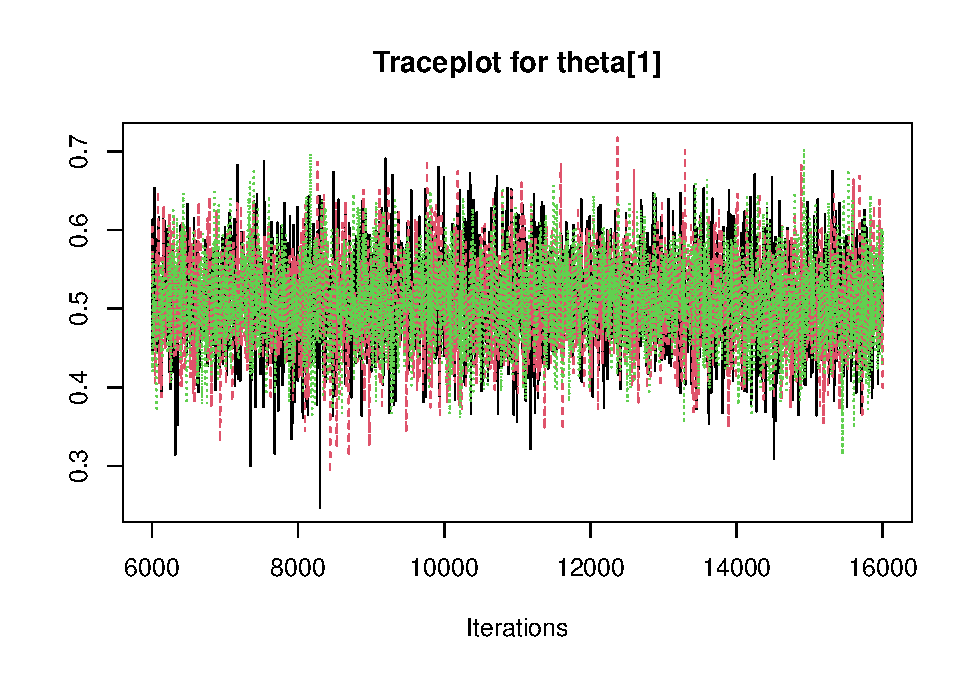
\includegraphics{Final-Project_files/figure-latex/appendix-code-2-1.pdf}
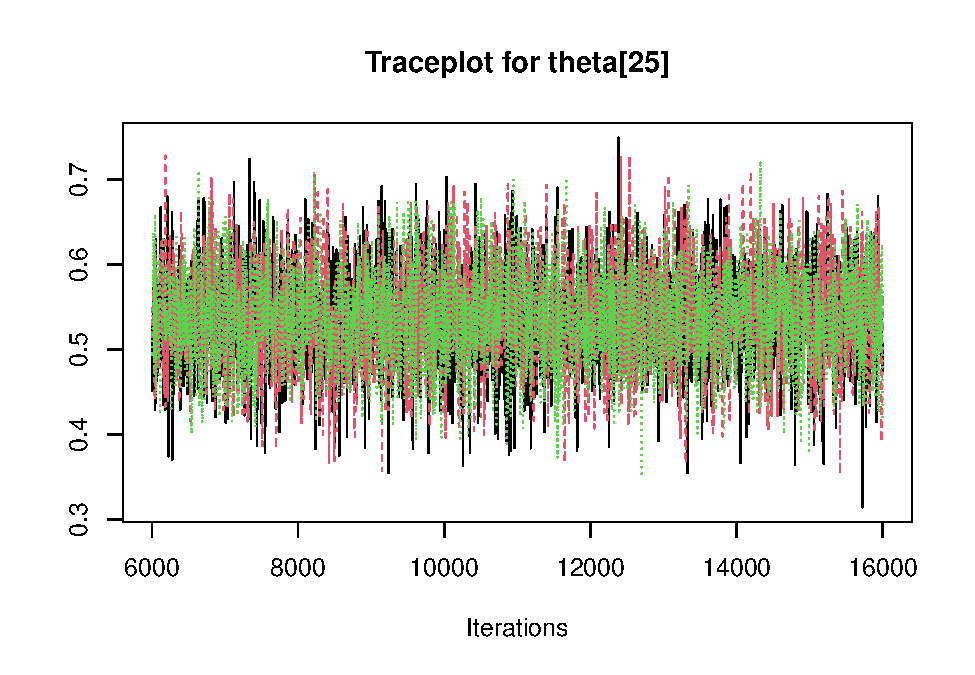
\includegraphics{Final-Project_files/figure-latex/appendix-code-2-2.pdf}
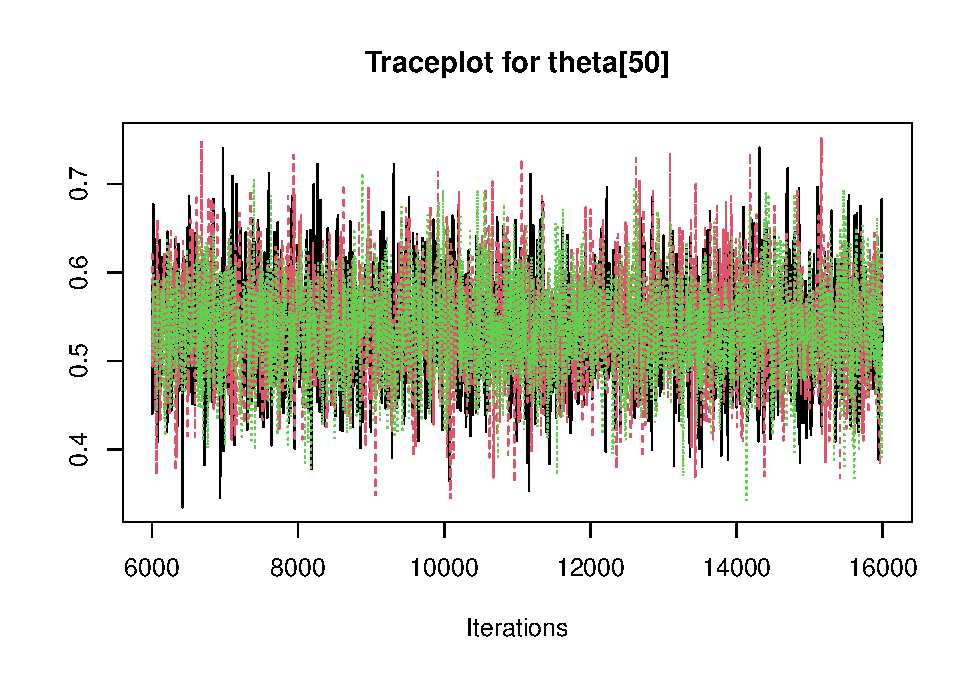
\includegraphics{Final-Project_files/figure-latex/appendix-code-2-3.pdf}
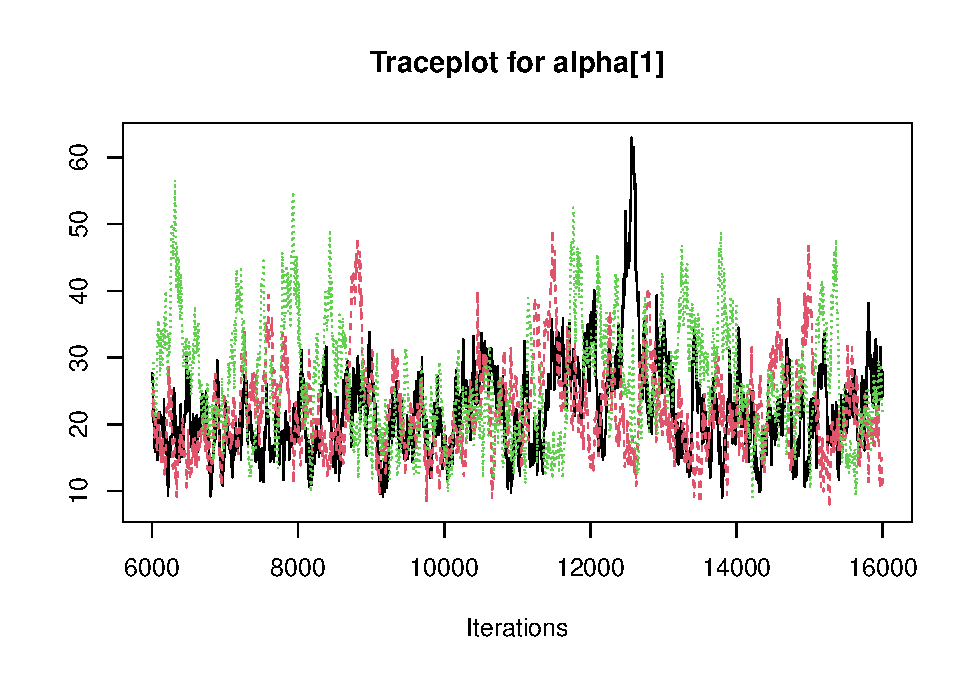
\includegraphics{Final-Project_files/figure-latex/appendix-code-2-4.pdf}
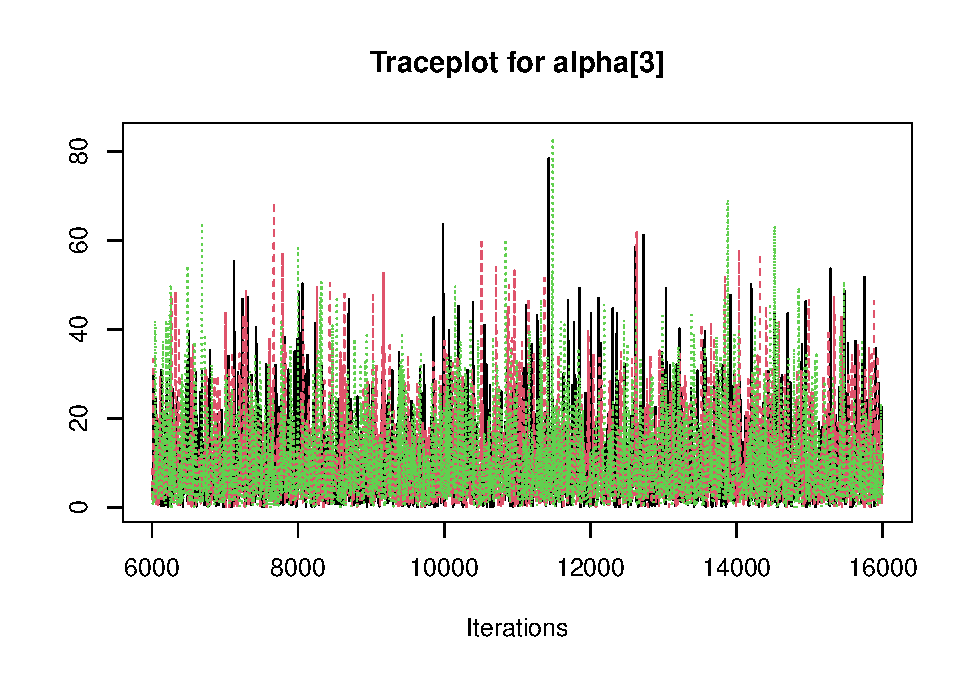
\includegraphics{Final-Project_files/figure-latex/appendix-code-2-5.pdf}
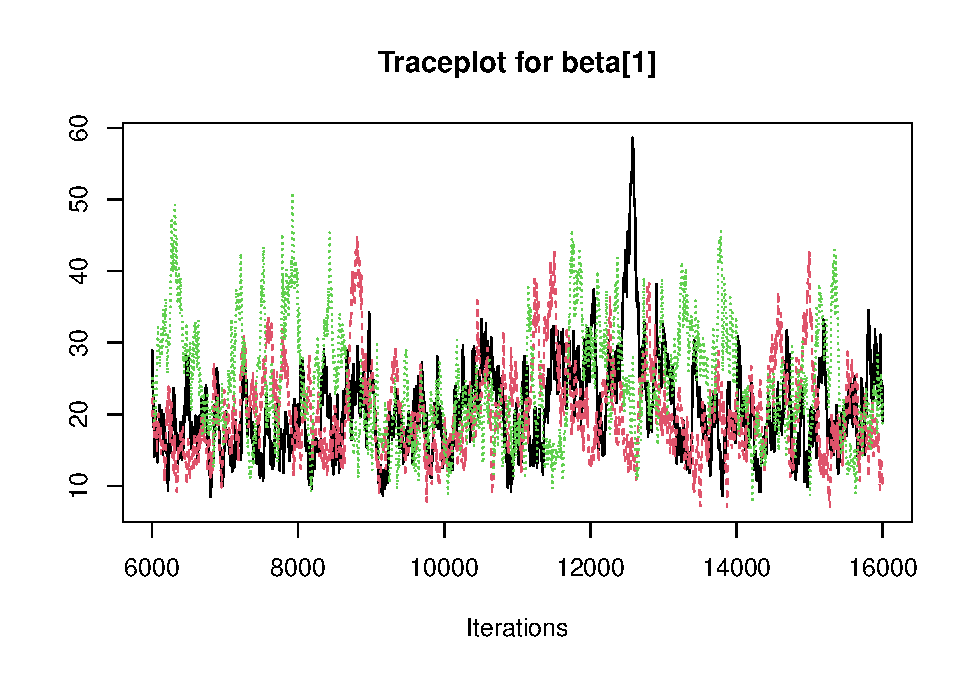
\includegraphics{Final-Project_files/figure-latex/appendix-code-2-6.pdf}
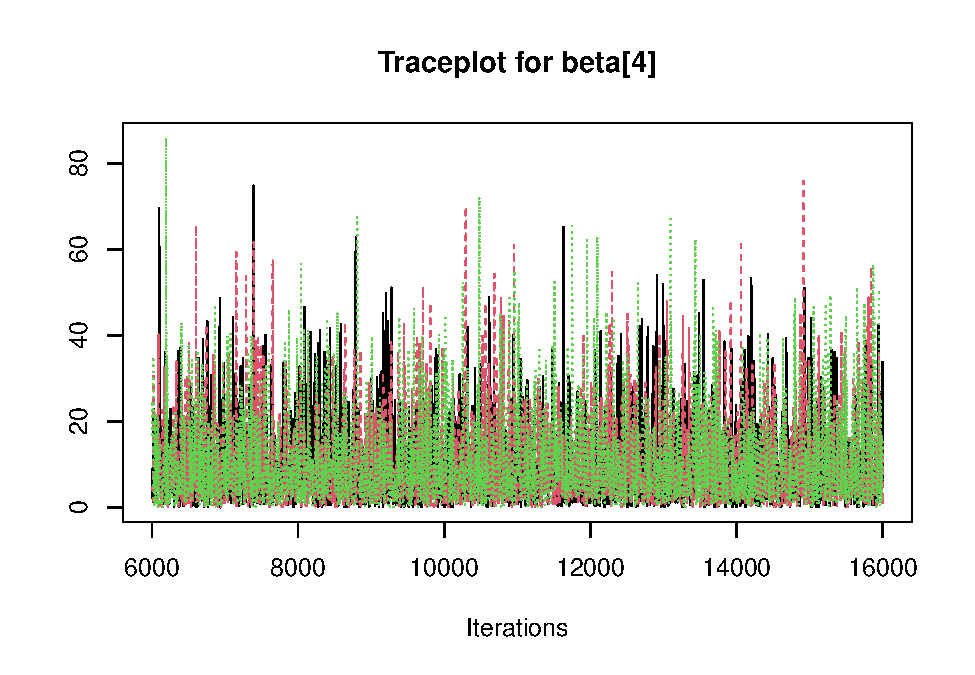
\includegraphics{Final-Project_files/figure-latex/appendix-code-2-7.pdf}

\begin{Shaded}
\begin{Highlighting}[]
\CommentTok{\# Effective Sample Size (ESS) for selected parameters}
\NormalTok{ess\_subset }\OtherTok{\textless{}{-}} \FunctionTok{effectiveSize}\NormalTok{(samples[, selected\_params])}
\NormalTok{ess\_table }\OtherTok{\textless{}{-}} \FunctionTok{data.frame}\NormalTok{(}
  \AttributeTok{Parameter =} \FunctionTok{names}\NormalTok{(ess\_subset),}
  \AttributeTok{ESS =} \FunctionTok{round}\NormalTok{(}\FunctionTok{as.numeric}\NormalTok{(ess\_subset), }\DecValTok{0}\NormalTok{)}
\NormalTok{)}
\FunctionTok{print}\NormalTok{(ess\_table)}
\end{Highlighting}
\end{Shaded}

\begin{verbatim}
##   Parameter  ESS
## 1  theta[1] 6279
## 2 theta[25] 5787
## 3 theta[50] 5766
## 4  alpha[1]  164
## 5  alpha[3] 6000
## 6   beta[1]  149
## 7   beta[4] 6423
\end{verbatim}

\begin{Shaded}
\begin{Highlighting}[]
\CommentTok{\# ACF plots one by one}
\ControlFlowTok{for}\NormalTok{ (param }\ControlFlowTok{in}\NormalTok{ selected\_params) \{}
  \FunctionTok{acf}\NormalTok{(samples\_combined[, param], }\AttributeTok{main =} \FunctionTok{paste}\NormalTok{(}\StringTok{"ACF for"}\NormalTok{, param))}
\NormalTok{\}}
\end{Highlighting}
\end{Shaded}

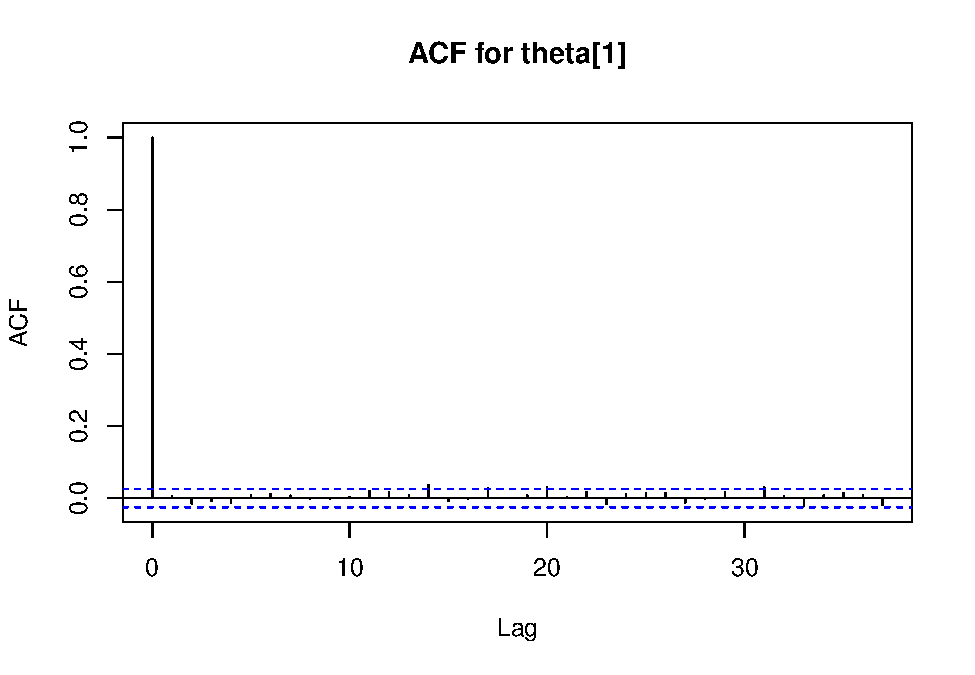
\includegraphics{Final-Project_files/figure-latex/appendix-code-2-8.pdf}
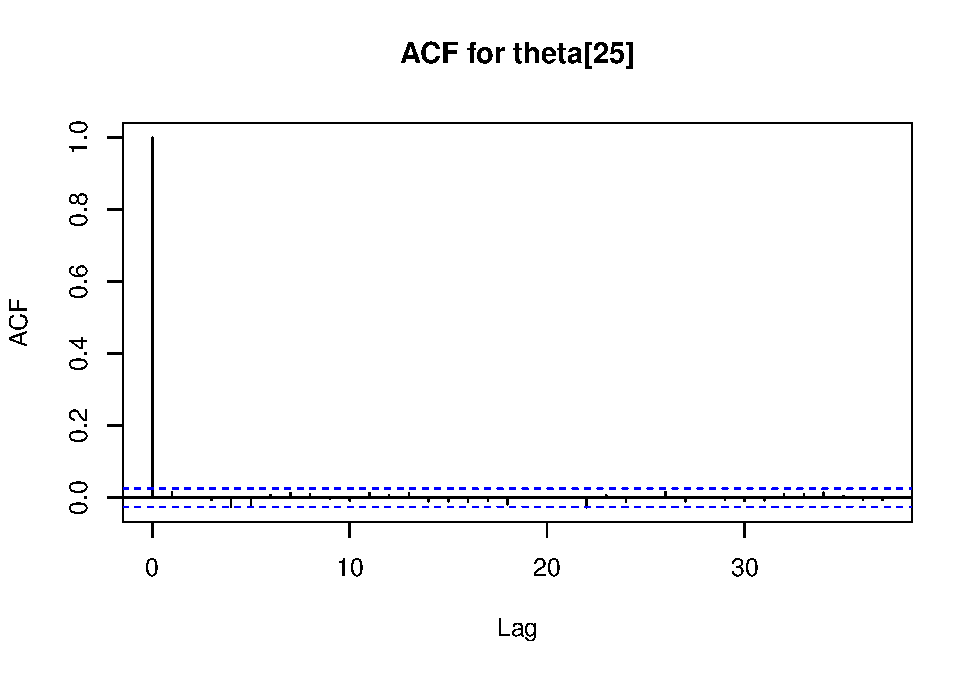
\includegraphics{Final-Project_files/figure-latex/appendix-code-2-9.pdf}
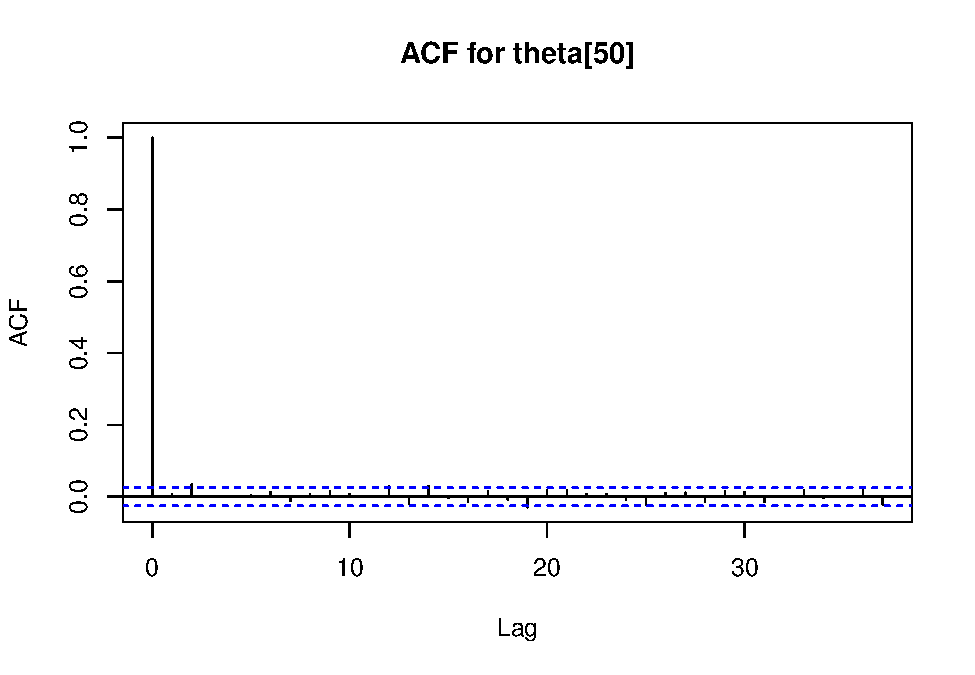
\includegraphics{Final-Project_files/figure-latex/appendix-code-2-10.pdf}
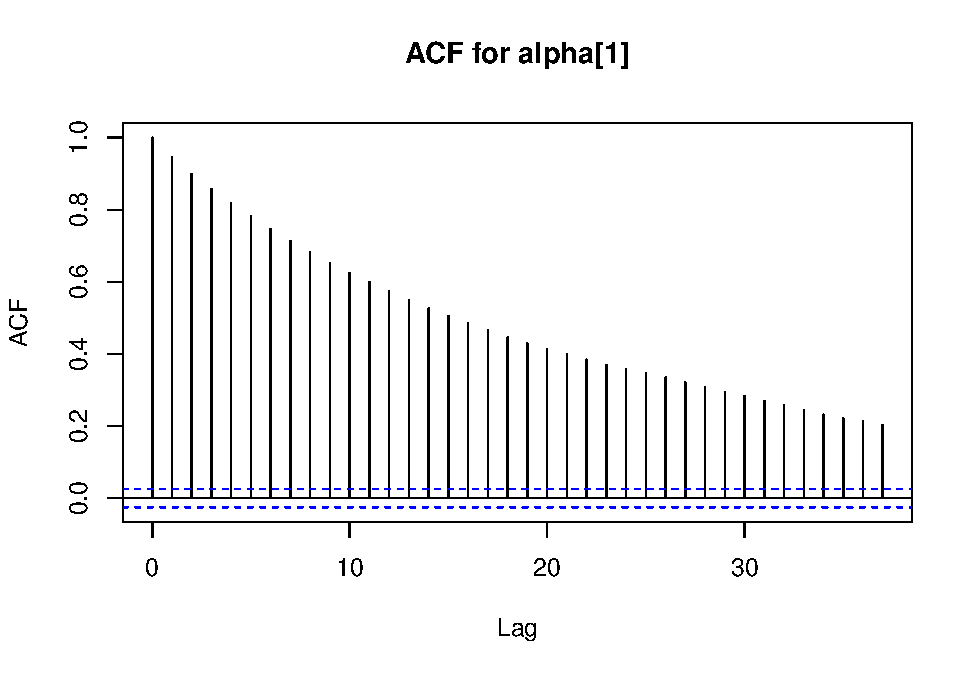
\includegraphics{Final-Project_files/figure-latex/appendix-code-2-11.pdf}
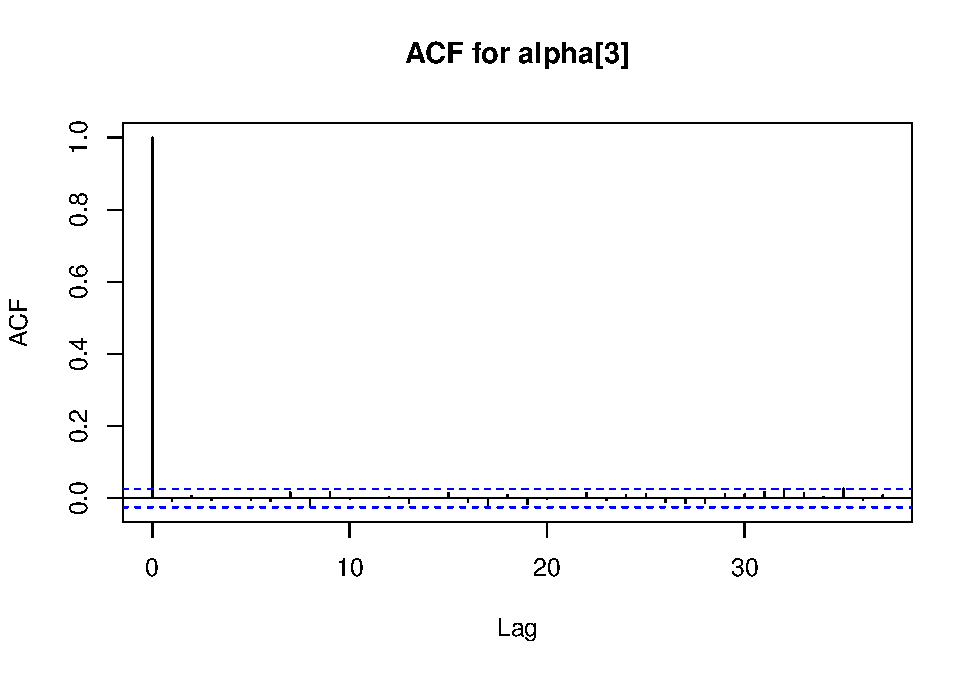
\includegraphics{Final-Project_files/figure-latex/appendix-code-2-12.pdf}
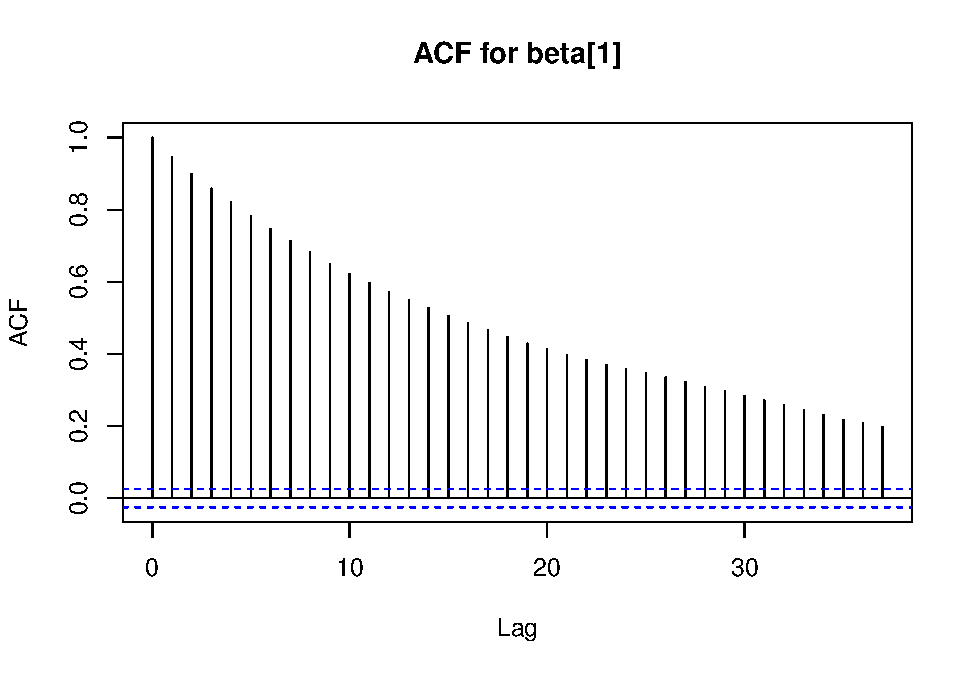
\includegraphics{Final-Project_files/figure-latex/appendix-code-2-13.pdf}
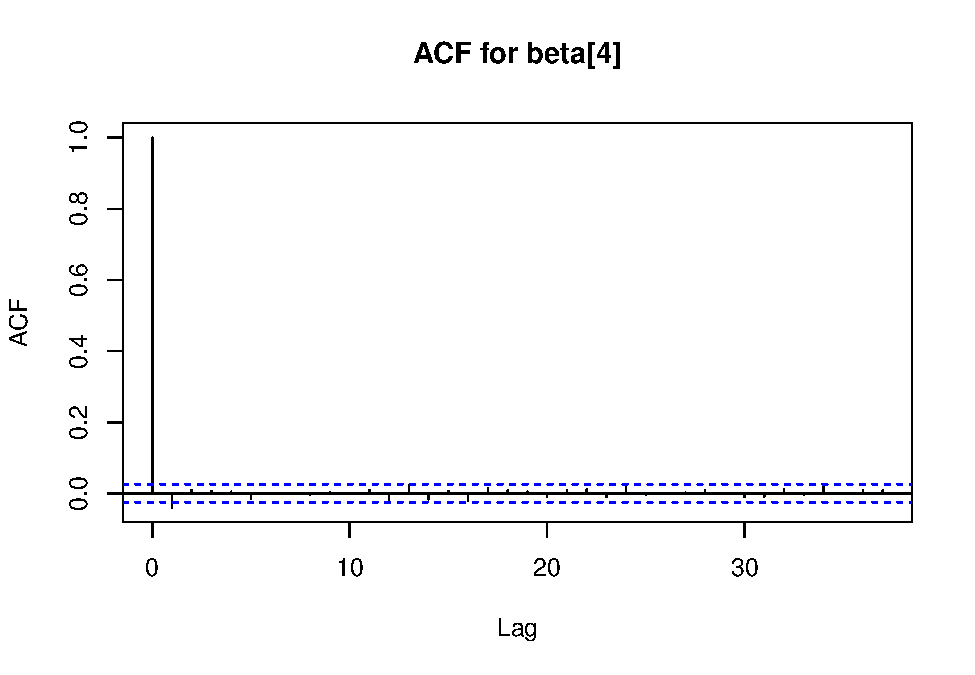
\includegraphics{Final-Project_files/figure-latex/appendix-code-2-14.pdf}

\subsection{Result Summary}\label{result-summary}

\begin{Shaded}
\begin{Highlighting}[]
\CommentTok{\# samples\_combined has all MCMC draws}

\CommentTok{\# Extract only theta samples}
\NormalTok{theta\_samples }\OtherTok{\textless{}{-}}\NormalTok{ samples\_combined[, }\FunctionTok{grep}\NormalTok{(}\StringTok{"\^{}theta"}\NormalTok{, }\FunctionTok{colnames}\NormalTok{(samples\_combined))]}

\CommentTok{\# Calculate posterior mean for each stock}
\NormalTok{posterior\_means\_theta }\OtherTok{\textless{}{-}} \FunctionTok{colMeans}\NormalTok{(theta\_samples)}

\CommentTok{\# Make a dataframe for stocks}
\NormalTok{posterior\_summary }\OtherTok{\textless{}{-}} \FunctionTok{data.frame}\NormalTok{(}
  \AttributeTok{stockID =} \DecValTok{1}\SpecialCharTok{:}\DecValTok{50}\NormalTok{,}
  \AttributeTok{posterior\_mean\_theta =}\NormalTok{ posterior\_means\_theta}
\NormalTok{)}

\CommentTok{\# Recover sector and stock number inside sector}
\NormalTok{posterior\_summary}\SpecialCharTok{$}\NormalTok{sector }\OtherTok{\textless{}{-}} \FunctionTok{ceiling}\NormalTok{(posterior\_summary}\SpecialCharTok{$}\NormalTok{stockID }\SpecialCharTok{/} \DecValTok{10}\NormalTok{)}
\NormalTok{posterior\_summary}\SpecialCharTok{$}\NormalTok{stock }\OtherTok{\textless{}{-}}\NormalTok{ posterior\_summary}\SpecialCharTok{$}\NormalTok{stockID }\SpecialCharTok{{-}}\NormalTok{ (posterior\_summary}\SpecialCharTok{$}\NormalTok{sector }\SpecialCharTok{{-}} \DecValTok{1}\NormalTok{) }\SpecialCharTok{*} \DecValTok{10}

\CommentTok{\# View the summary}
\FunctionTok{print}\NormalTok{(posterior\_summary)}
\end{Highlighting}
\end{Shaded}

\begin{verbatim}
##           stockID posterior_mean_theta sector stock
## theta[1]        1            0.5111606      1     1
## theta[2]        2            0.4964088      1     2
## theta[3]        3            0.5242340      1     3
## theta[4]        4            0.5108416      1     4
## theta[5]        5            0.5530283      1     5
## theta[6]        6            0.4971426      1     6
## theta[7]        7            0.5528694      1     7
## theta[8]        8            0.6072761      1     8
## theta[9]        9            0.4831754      1     9
## theta[10]      10            0.6081898      1    10
## theta[11]      11            0.4702009      2     1
## theta[12]      12            0.4831783      2     2
## theta[13]      13            0.5654058      2     3
## theta[14]      14            0.5679584      2     4
## theta[15]      15            0.6074555      2     5
## theta[16]      16            0.5104895      2     6
## theta[17]      17            0.4423746      2     7
## theta[18]      18            0.4822784      2     8
## theta[19]      19            0.5109533      2     9
## theta[20]      20            0.4834284      2    10
## theta[21]      21            0.4684564      3     1
## theta[22]      22            0.5394026      3     2
## theta[23]      23            0.4568459      3     3
## theta[24]      24            0.4557436      3     4
## theta[25]      25            0.5384138      3     5
## theta[26]      26            0.5515056      3     6
## theta[27]      27            0.4988163      3     7
## theta[28]      28            0.5533650      3     8
## theta[29]      29            0.4280509      3     9
## theta[30]      30            0.5258278      3    10
## theta[31]      31            0.5674537      4     1
## theta[32]      32            0.4841585      4     2
## theta[33]      33            0.5399082      4     3
## theta[34]      34            0.4974535      4     4
## theta[35]      35            0.4706638      4     5
## theta[36]      36            0.5112278      4     6
## theta[37]      37            0.5526852      4     7
## theta[38]      38            0.4981398      4     8
## theta[39]      39            0.5375287      4     9
## theta[40]      40            0.5392520      4    10
## theta[41]      41            0.5661348      5     1
## theta[42]      42            0.4829654      5     2
## theta[43]      43            0.5242351      5     3
## theta[44]      44            0.5656187      5     4
## theta[45]      45            0.4569388      5     5
## theta[46]      46            0.5525250      5     6
## theta[47]      47            0.5395215      5     7
## theta[48]      48            0.5388983      5     8
## theta[49]      49            0.5118490      5     9
## theta[50]      50            0.5387058      5    10
\end{verbatim}

\begin{Shaded}
\begin{Highlighting}[]
\CommentTok{\# Sector{-}level average posterior mean}
\NormalTok{sector\_summary\_post }\OtherTok{\textless{}{-}}\NormalTok{ posterior\_summary }\SpecialCharTok{\%\textgreater{}\%}
  \FunctionTok{group\_by}\NormalTok{(sector) }\SpecialCharTok{\%\textgreater{}\%}
  \FunctionTok{summarize}\NormalTok{(}\AttributeTok{sector\_mean\_theta =} \FunctionTok{mean}\NormalTok{(posterior\_mean\_theta))}

\FunctionTok{print}\NormalTok{(sector\_summary\_post)}
\end{Highlighting}
\end{Shaded}

\begin{verbatim}
## # A tibble: 5 x 2
##   sector sector_mean_theta
##    <dbl>             <dbl>
## 1      1             0.534
## 2      2             0.512
## 3      3             0.502
## 4      4             0.520
## 5      5             0.528
\end{verbatim}

\begin{Shaded}
\begin{Highlighting}[]
\CommentTok{\# Identify best sector}
\NormalTok{best\_sector }\OtherTok{\textless{}{-}}\NormalTok{ sector\_summary\_post }\SpecialCharTok{\%\textgreater{}\%}
  \FunctionTok{filter}\NormalTok{(sector\_mean\_theta }\SpecialCharTok{==} \FunctionTok{max}\NormalTok{(sector\_mean\_theta))}

\FunctionTok{print}\NormalTok{(best\_sector)}
\end{Highlighting}
\end{Shaded}

\begin{verbatim}
## # A tibble: 1 x 2
##   sector sector_mean_theta
##    <dbl>             <dbl>
## 1      1             0.534
\end{verbatim}

\begin{Shaded}
\begin{Highlighting}[]
\CommentTok{\# Identify best stock within each sector}
\NormalTok{best\_stock\_each\_sector }\OtherTok{\textless{}{-}}\NormalTok{ posterior\_summary }\SpecialCharTok{\%\textgreater{}\%}
  \FunctionTok{group\_by}\NormalTok{(sector) }\SpecialCharTok{\%\textgreater{}\%}
  \FunctionTok{filter}\NormalTok{(posterior\_mean\_theta }\SpecialCharTok{==} \FunctionTok{max}\NormalTok{(posterior\_mean\_theta))}

\FunctionTok{print}\NormalTok{(best\_stock\_each\_sector)}
\end{Highlighting}
\end{Shaded}

\begin{verbatim}
## # A tibble: 5 x 4
## # Groups:   sector [5]
##   stockID posterior_mean_theta sector stock
##     <int>                <dbl>  <dbl> <dbl>
## 1      10                0.608      1    10
## 2      15                0.607      2     5
## 3      28                0.553      3     8
## 4      31                0.567      4     1
## 5      41                0.566      5     1
\end{verbatim}

\end{document}
